\documentclass[letterpaper,12pt]{article}
\usepackage[utf8]{inputenc}

\usepackage{rotating}
\usepackage[top=1in, bottom=1in, left=1in, right=1in]{geometry}
\usepackage{graphicx}
\usepackage[numbers,square,sort&compress]{natbib}
\usepackage{setspace}
\usepackage[cdot,mediumqspace,]{SIunits}
\usepackage{hyperref}
\usepackage{mathtools}
\usepackage{url}
\usepackage{authblk}
\usepackage{placeins}
\usepackage{float}

\onehalfspacing
\title{Computational Physics Lab 09}
\author{Anita Bahmanyar}
\affil{\small {Student Number: 998909098}}
\date{November 7, 2014}

\usepackage{graphicx}

\renewcommand\thesubsection{\alph{subsection}}

\begin{document}

\maketitle

\section*{Q2}

%figure a
\FloatBarrier
\begin{figure}[H]
\centering
\includegraphics[scale=0.55]{q2_a.png}
\caption{}
\end{figure}
\FloatBarrier

%figure b
\FloatBarrier
\begin{figure}[H]
\centering
\includegraphics[scale=0.55]{q2_c.png}
\caption{}
\end{figure}
\FloatBarrier

%figure c
\FloatBarrier
\begin{figure}[H]
\centering
\includegraphics[scale=0.55]{q2_b.png}
\caption{}
\end{figure}
\FloatBarrier


\section*{Q3}

\FloatBarrier
\begin{figure}[H]
\centering
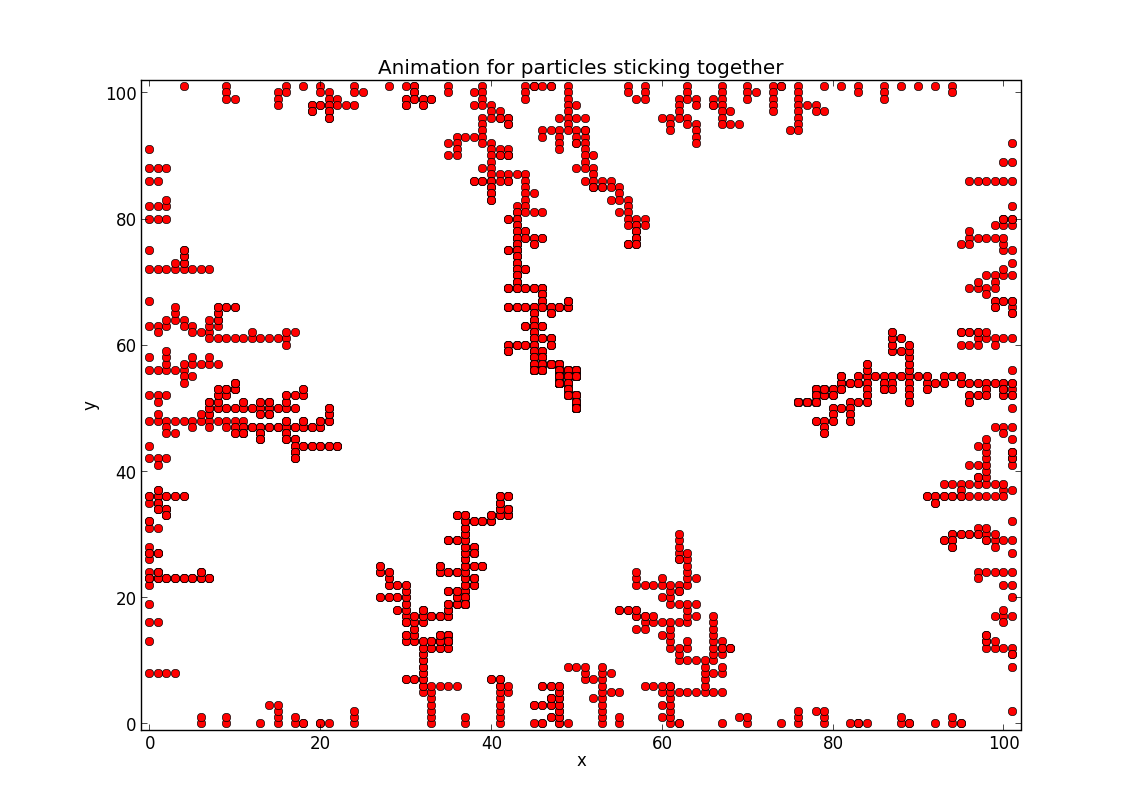
\includegraphics[scale=0.6]{q3.png}
\caption{}
\end{figure}
\FloatBarrier


\section*{Q4}

%figure a
\FloatBarrier
\begin{figure}[H]
\centering
\includegraphics[scale=0.5]{q4_a.png}
\caption{}
\end{figure}
\FloatBarrier

%figure b
\FloatBarrier
\begin{figure}[H]
\centering
\includegraphics[scale=0.5]{q4_b.png}
\caption{}
\end{figure}
\FloatBarrier

%figure c
\FloatBarrier
\begin{figure}[H]
\centering
\includegraphics[scale=0.5]{q4_c.png}
\caption{}
\end{figure}
\FloatBarrier


\end{document}


